\chapter{Identifikácia jednonukleotidových polymorfizmov}

\label{kap:identifikacia_SNP} 

V tejto časti navrhneme techniku na odhaľovanie jednonukleotidových
polymorfizmov (SNP) v sekvenovaných dátach. Uvažujeme pritom najjednoduchší
možný scenár, keď sekvenovaná vzorka neobsahuje žiadne iné varianty a jednotlivé
SNPy nie sú príliš blízko seba. Predpokladáme teda, že ak sa sekvenovaná vzorka 
líši od referencie v nejakej báze, v okolitých bázach sa tieto dve sekvencie
zhodujú. Náš postup pri spracovaní jedného čítania sa skladá z troch fáz:

\begin{enumerate}
\item Zistenie, ktorej časti referencie toto čítanie zopovedá.
\item Približné zarovnanie signálu k bázam referencie.
\item Odhadnutie pravdepodobnosti SNPu na jednotlivých pozíciách sekvencie.
\end{enumerate}

Na riešenie prvých dvoch fáz používame existujúce nástroje, jadro našej práce je
zamerané na tretiu fázu.

\section{Rámcové zarovnanie čítania k referencii}
\label{ramcove_zarovnanie}
Keďže čítania, s ktorými pracujeme, nemusia zodpovedať celej referencii (môže ísť o
kratšie fragmenty sekvenovanej DNA), v prvej fáze spracovania každého čítania
je naším cieľom zistiť, ktorej časti referencie zodpovedá. To robíme v dvoch krokoch:

\begin{enumerate}
\item \label{item:basecall} Pomocou basecallera preložíme signál v našom čítaní do DNA sekvencie.
\item \label{item:zarovnanie_baz} Nájdeme časť referencie, ktorá sa tejto sekvencii najviac podobá.
\end{enumerate}

Na realizáciu kroku \ref{item:basecall} používame basecaller Albacore poskytovaný priamo výrobcom sekvenátora MinION.
Presnosť tohto basecallera sa pohybuje v rozmedzí $85\%$ až $90\%$ \cite{BasecallerComparison},
výstup teda nebude úplne presne zodpovedať sekvenovanej
DNA. V praxi je však takáto presnosť na krok \ref{item:zarovnanie_baz} väčšinou dostatočná.
Problém, ktorý riešime v kroku \ref{item:zarovnanie_baz}, je známy ako
\emph{zarovnanie sekvencií}. Na zarovnávanie sekvencií v tejto práci používame
nástroj BWA-MEM \cite{BWA-MEM}.

\section{Približné zarovnanie signálu}
\label{sec:resquiggle}

Po dokončení prvej fázy už vieme, ktorej časti referencie
by malo zodpovedať spracovávané čítanie. Stále však nevieme, ktoré časti nameraného signálu
zodpovedajú jednotlivým bázam v referencii. Aproximáciu tohoto priradenia (zarovnania signálu k 
referencii)
získame pomocou nástroja \resquiggle{} z balíčka tombo \cite{tombo}. 

Nástroj \resquiggle{} surový signál normalizuje použitím mediánovej normalizácie, ktorú vo
svojej práci \cite{Stoiber2017} popisuje Stoiber et. al.
S takto znormalizovaným signálom budeme pracovať aj vo zvyšku našej práce.

Po znormalizovaní si \resquiggle{} rozdelí signál na udalosti, čo sú úseky, kde je hodnota signálu zhruba
konštantná. Pre každý úsek vypočíta priemernú hodnotu signálu v ňom.
Pomocou dynamického programovania, konkrétne algoritmu z triedy \emph{dynamic time warping}, potom vypočíta 
najvierohodnejšie priradenie udalostí k bázam \cite{resquiggle}. 
Vierohodnosť daného priradenia je hodnotená pomocou modelu pre očakávané hodnoty signálu pri
jednotlivých \kmer{och}. Tento model pre fixné $k$ (v praxi väčšinou $k=5$ alebo $k=6$)
obsahuje pre každý zo $4^k$ možných \kmer{ov} informáciu, akú hodnotu signálu
očakávame, ak daný \kmer{} práve prechádza nanopórom.


Pri zarovnávaní \resquiggle{} predpokladá, že signál z nášho čítania presne zodpovedá referencii.
Keďže sekvenovaná postupnosť obsahuje aj varianty, dá sa očakávať, že v okolí týchto variantov
zarovnanie nebude veľmi presné. Dá sa však použiť ako aproximácia, v okolí ktorej budeme hľadať
presnejšie zarovnanie.

\section{Pravdepodobnosť SNPu na jednej pozícii}
\label{sec:jedna_pozicia}

Pri hľadaní SNPov v sekvenovanej DNA sa pre každú pozíciu v referencii snažíme odhadnúť, či je
na tejto pozícii v sekvenovanej postupnosti rovnaká báza ako v referencii alebo je tam SNP. Uvažujeme
preto štyri hypotézy. Prvá hypotéza je, že v sekvenovanej postupnosti je na skúmanej
pozícii \texttt{A} a na okolitých pozíciách rovnaké bázy ako v referencii. Zvyšné tri hypotézy sú
analogické, s \texttt{C}, \texttt{G} a \texttt{T}. Jedna z hypotéz teda vždy hovorí, že na danej
pozícii nie je variant, zvyšné tri tvrdia, že sa na tejto pozícii nachádza SNP.

\todo{obrázok}

Pre každú zo štyroch hypotéz ohodnotíme, ako dobre vysvetľuje signál nameraný v okolí skúmanej
pozície. Vezmeme výsek $T$ z referencie obsahujúci skúmanú pozíciu s okolím niekoľkých báz a úsek $S$
z nameraného signálu, ktorý tejto časti referencie zodpovedá podľa približného zarovnania 
z kapitoly \ref{sec:resquiggle}. V postupnosti $T$ zmeníme bázu na skúmanej pozícii na tú, ktorá 
tam má byť podľa našej hypotézy. Takto upravenú postupnosť označme $D_B$, kde $B$ je báza, ktorú
máme v našej hypotéze na skúmanej pozícii. 
Následne vypočítame podmienenú pravdepodobnosť $P(S ~|~ D_B)$, že by postupnosť báz $D_B$ pri sekvenovaní vygenerovala signál $S$.

\subsection{Pravdepodobnostný model}

Podmienené pravdepodobnosti, že by nejaká postupnosť báz $D$ pri sekvenovaní vygenerovala signál $S$,
budú definované jednoduchým pravdepodobnostným modelom.

Model predpokladá, že bázy sekvenovaného vlákna DNA postupne prechádzajú nanopórom, pričom
každá báza sa v nanopóre nachádza počas minimálne $M$ po sebe idúcich meraní signálu. Ku každej
nameranej hodnote signálu teda môžeme priradiť bázu, ktorá sa v danom čase nachádzala v nanopóre.
Tomuto priradeniu budeme hovoriť \emph{zarovnanie signálu}.

\begin{definicia}

Nech $n, m, M \in \mathbb{Z}^+$, pričom $m \geq n M$. \emph{Zarovnaním signálu dĺžky $m$ k sekvencii
o dĺžke $n$ s
 minimálnou dĺžkou udalosti $M$} nazývame ľubovoľné zobrazenie $f: \{0, 1, \dots, m-1\} \rightarrow \{0, 1, \dots, n-1\}$
také, že:

\begin{itemize}
\item $f$ je neklesajúce, teda $\forall x, y \in \{0, 1, \dots, m-1\}: x < y \Rightarrow f(x) \leq f(y)$.
\item $\forall i \in \{0, 1, \dots, n-1\}: \abs*{\{x ~|~ f(x) = i\}} \geq M$.
\end{itemize}

Množinu všetkých zarovnaní signálu dĺžky $m$ k sekvencii o dĺžke $n$ s minimálnou dĺžkou udalosti $M$ budeme označovať ako
$A(n, m, M)$.

\end{definicia}

Náš model predpokladá, že nameraný signál závisí iba od bázy, ktorá je práve v nanopóre, $c_1$
báz pred ňou a $c_2$ báz za ňou. To sa nedá aplikovať na prvých $c_1$ a posledných $c_2$ báz 
sekvenovanej postupnosti. Pri modelovaní preto budeme pre jednoduchosť predpokladať, že DNA postupnosť, 
ktorej signál modelujeme, išla cez nanopór ako súčasť nejakej dlhšej sekvencie. Na modelovanie
signálu, ktorý bol pri tejto postupnosti zaznamenaný, budeme teda potrebovať poznať aj 
kontext $c_1$ báz pred začiatkom postupnosti a $c_2$ báz za jej koncom.

\begin{definicia}

\emph{DNA sekvenciou dĺžky $n$ s kontextom $c_1$ a $c_2$} nazývame ľubovoľné zobrazenie 
$D: \{-c_1, -c_1+1, \dots, n-1+c_2\} \rightarrow \bazy$. Funkčnú hodnotu $D$ v danom bode $i$
budeme namiesto $D(i)$ značiť ako $D_i$.

\end{definicia}

Nech $k = c_1 + 1 + c_2$. Budeme hovoriť, že nejaký \kmer{} sa nachádza v nanopóre, ak báza, 
ktorá je v nanopóre, spolu s okolím $c_1$ báz pred ňou a $c_2$ báz za ňou tvorí tento \kmer{}.

Úroveň signálu závisí v našom modeli od \kmer{u}, ktorý sa v čase merania nachádza v nanopóre.
Pre každý zo $4^k$ možných \kmer{ov} uvažujeme rozdelenie 
pravdepodobnosti pre hodnotu signálu.
Keďže pracujeme s digitalizovanou hodnotou signálu, existuje iba konečné množstvo hodnôt, ktoré
môže signál nadobudnúť. Rozdelenie pravdepodobnosti teda bude pravdepodobnostná funkcia.

\begin{definicia}

Množinu všetkých možných nameraných hodnôt signálu budeme označovať $\mathbb{S}$.

\end{definicia}

Čísla $M$, $c_1$, $c_2$ a pravdepodobnostné funkcie pre jednotlivé \kmer{y} sú jediné
parametre nášho modelu.

\begin{definicia}

\emph{\kmer{ový} model} je štvorica $(M, c_1, c_2, \Delta)$, kde:

\begin{itemize}
\item $M \in \mathbb{Z}^+$.
\item $c_1, c_2 \in \mathbb{Z}_{\geq 0}$.
\item $\Delta$ je množina, ktorá pre každé $K \in \bazy^{c_1 + 1 + c_2}$ obsahuje rozdelenie pravdepodobnosti
$\delta_K$ nad množinou $\mathbb{S}$.
\end{itemize}
\end{definicia}

V našom modeli budeme jednotlivé merania považovať za nezávislé udalosti.

\begin{definicia}

Nech $(M, c_1, c_2, \Delta)$ je \kmer{ový} model, $n, m \in \mathbb{Z}^+$, $D$ je DNA sekvencia dĺžky $n$ s konextom
$c_1$ a $c_2$, nech $S = (S_i)_{i=0}^{m-1}$ je postupnosť hodnôt z $\mathbb{S}$ a nech 
$a \in A(n, m, M)$. Pravdepodobnosť vygenerovania signálu $S$ pri prechode sekvencie $D$ nanopórom
pri zarovnaní $a$ podľa modelu $(M, c_1, c_2, \Delta)$ bude:

$$P(S ~|~ D, a) = \prod\limits_{i=0}^{m-1} \delta_{(D_{a(i)-c_1}, \dots, D_{a(i)+c_2})}(S_i) \text{.}$$

\end{definicia}

Výslednú podmienenú pravdepodobnosť $P(S ~|~ D)$ získame marginalizáciou zarovnania $a$.
 Pre jednoduchosť budeme predpokladať, že všetky zarovnania z $A(n, m, M)$ sú rovnako pravdepodobné.

\begin{definicia}

Nech $(M, c_1, c_2, \Delta)$ je \kmer{ový} model, $n, m \in \mathbb{Z}^+$, $D$ je DNA sekvencia dĺžky $n$ s kontextom $c_1$ a $c_2$ a nech $S = (S_i)_{i=0}^{m-1}$ je postupnosť hodnôt z $\mathbb{S}$.
Pravdepodobnosť vygenerovania signálu $S$ pri sekvenovaní $D$ podľa modelu $(M, c_1, c_2, \Delta)$ je:

$$P(S ~|~ D) =  \frac{\sum\limits_{a \in A(n, m, M)} P(S ~|~ D, a)}{\abs*{A(n, m, M)}} \text{.}$$
\end{definicia}



\subsection{Výpočet podmienenej pravdepodobnosti}
\label{sec:dtw}

Balík nástrojov tombo obsahuje aj rozdelenia pravdepodobnosti signálu pre jednotlivé \kmer{y} (konkrétne pre $k=6$ a
$c_1 = 2$). Tombo modeluje rozdelenie pre každý \kmer{} ako normálne rozdelenie. Parametre týchto normálnych rozdelení
sa pre jednotlivé \kmer{y} líšia a boli odhadnuté empiricky na základe dát. 

Keďže ide o hustotu pravdepodobnosti a nie pravdepodobnostnú funkciu, nemôžeme rozdelenia z tombo priamo použiť
ako funkcie $\delta$ z nášho modelu. Označme distribúciu z tombo pre \kmer{} $K$ ako $\theta_K$. Najmenší možný rozdiel,
ktorý môžu mať dve hodnoty signálu po digitalizácii, označme $r$. V našom modeli potom pre \kmer{} $K$ použijeme
pravdepodobnostnú funkciu $\delta_K$ definovanú ako:

$$\delta_K(x) = \int\limits_{x-r/2}^{x+r/2} \theta_K(t) \diff t \text{,}$$

ktorú aproximujeme ako:

$$\delta_K(x) = r \cdot \theta_K(x) \text{.}$$

Podmienenú pravdepodobnosť vygenerovania signálu $S$ dĺžky $m$ pri sekvenovaní postupnosti $D$ dĺžky $n$ s kontextom 
$c_1$ a $c_2$ teda budeme počítať ako:

\begin{multline*}
P(S ~|~ D) = \frac{\sum\limits_{a \in A(n, m, M)} \prod\limits_{i=0}^{m-1} r \cdot \theta_{(D_{a(i)-c_1}, \dots, D_{a(i)+c_2})}(S_i)}{\abs*{A(n, m, M)}} = \\
= \frac{r^m}{\abs*{A(n, m, M)}} \sum\limits_{a \in A(n, m, M)} \prod\limits_{i=0}^{m-1} \theta_{(D_{a(i)-c_1}, \dots, D_{a(i)+c_2})}(S_i) \text{.} 
\end{multline*}

Pri vyhodnocovaní hypotéz pre jednu pozíciu pracujeme stále s rovnako dlhou postupnosťou báz a s tým istým úsekom signálu, teda hodnoty
$r^m$ a $\abs*{A(n, m, M)}$ sú pre všetky štyri hypotézy rovnaké. Keďže pri týchto podmienených pravdepodobnostiach bude dôležitý iba ich
pomer, v našej implementácii počítame iba hodnotu

$$\sum\limits_{a \in A(n, m, M)} \prod\limits_{i=0}^{m-1} \theta_{(D_{a(i)-c_1}, \dots, D_{a(i)+c_2})}(S_i) \text{.}$$

Naivný výpočet tejto sumy by bol pomalý, preto ju počítame dynamickým programovaním.
Používame algoritmus z rodiny označovanej ako \emph{dynamic time warping}. Algoritmy tohto typu sa používajú, keď chceme zistiť,
ktoré časti dvoch postupností si vzájomne zodpovedajú \cite{DynamicTimeWarping}.

Pre každé $x \in \{0, 1, \dots, m\}, y \in \{0, 1, \dots, n\}$ vypočítame hodnotu

$$\textrm{DP}[y][x] = \sum\limits_{a \in A(y, x, M)} \prod\limits_{i=0}^{x-1} \theta_{(D_{a(i)-c_1}, \dots, D_{a(i)+c_2})}(S_i) \text{.}$$

Hodnota $\textrm{DP}[y][x]$ teda zodpovedá podmienenej pravdepodobnosti, že by prvých $y$ báz postupnosti $D$ vygenerovalo prvých $x$ hodnôt signálu.
Zjavne platí:
\begin{itemize}
\item $\textrm{DP}[0][0] = 1$
\item $\textrm{DP}[0][x] = 0$ pre $x \geq 1$
\item $\textrm{DP}[y][x] = 0$ pre $x < y M$
\end{itemize} 

Pre $y \geq 1$ a $x \geq y M$ môžeme množinu zarovnaní $A(y, x, M)$ rozdeliť na dve časti:

\begin{itemize}

\item $B(y, x, M) = \{a \in A(y, x, M) ~|~ \abs*{\{i ~|~ a(i) = y-1\}} = M\}$
\item $C(y, x, M) = \{a \in A(y, x, M) ~|~ \abs*{\{i ~|~ a(i) = y-1\}} > M\}$

\end{itemize}

Množina $B(y, x, M)$ obsahuje tie zarovnania, v ktorých je posledná báza priradená presne $M$ hodnotám signálu, množina $C(y, x, M)$ obsahuje
zarovnania, kde je posledná báza priradená ostro viac než $M$ hodnotám. Zjavne platí $B(y, x, M) \cap C(y, x, M) = \emptyset$ a vďaka podmienke,
že každá báza musí byť priradená aspoň $M$ hodnotám signálu platí aj $B(y, x, M) \cup C(y, x, M) = A(y, x, M)$. Sumu, ktorú počítame, preto
môžeme rozdeliť ako:

$$\textrm{DP}[y][x] = \sum\limits_{a \in B(y, x, M)} \prod\limits_{i=0}^{x-1} \theta_{(D_{a(i)-c_1}, \dots, D_{a(i)+c_2})}(S_i)
+ \sum\limits_{a \in C(y, x, M)} \prod\limits_{i=0}^{x-1} \theta_{(D_{a(i)-c_1}, \dots, D_{a(i)+c_2})}(S_i) \text{.}$$

Skrátením ľubovoľného zarovnania z $B(y, x, M)$ o posledných $M$ hodnôt (teda zúžením jeho definičného oboru na $\{0, \dots, x-M-1\}$)
dostaneme nejaké zarovnanie z $A(y-1, x-M, M)$. Toto skrátenie nám vlastne definuje bijekciu medzi $B(y, x, M)$ a $A(y-1, x-M, M)$. Prvú z našich dvoch
súm teda môžeme prepísať ako:

\begin{multline*}
\sum\limits_{a \in B(y, x, M)} \prod\limits_{i=0}^{x-1} \theta_{(D_{a(i)-c_1}, \dots, D_{a(i)+c_2})}(S_i) = \\
= \sum\limits_{a \in A(y-1, x-M, M)}\left( \prod\limits_{i=0}^{x-M-1} \theta_{(D_{a(i)-c_1}, \dots, D_{a(i)+c_2})}(S_i)  \prod\limits_{i=x-M}^{x-1}\theta_{(D_{y-1-c_1}, \dots, D_{y-1+c_2})}(S_i)\right) = \\
= \mathrm{DP}[y-1][x-M] \cdot \prod\limits_{i=x-M}^{x-1}\theta_{(D_{y-1-c_1}, \dots, D_{y-1+c_2})}(S_i) \text{.}
\end{multline*}

Skrátením ľubovoľného zarovnania z $C(y, x, M)$ o poslednú hodnotu dostaneme zarovnanie z $A(y, x-1, M)$, pričom opäť ide o bijekciu. Druhú sumu teda
môžeme prepísať ako:

\begin{multline*}
\sum\limits_{a \in C(y, x, M)} \prod\limits_{i=0}^{x-1} \theta_{(D_{a(i)-c_1}, \dots, D_{a(i)+c_2})}(S_i) = \\
= \sum\limits_{a \in A(y, x-1, M)} \theta_{(D_{y-1-c_1}, \dots, D_{y-1+c_2})}(S_{x-1}) \prod\limits_{i=0}^{x-2} \theta_{(D_{a(i)-c_1}, \dots, D_{a(i)+c_2})}(S_i)  = \\
= \mathrm{DP}[y][x-1] \cdot \theta_{(D_{y-1-c_1}, \dots, D_{y-1+c_2})}(S_{x-1}) \text{.}
\end{multline*}

Jednu hodnotu $\mathrm{DP}[y][x]$ teda vieme vypočítať z predošlých hodnôt v čase $O(M)$ ako:

\begin{align*}
\mathrm{DP}[y][x] =~ &\mathrm{DP}[y-1][x-M] \cdot \prod\limits_{i=x-M}^{x-1} \theta_{(D_{y-1-c_1}, \dots, D_{y-1+c_2})} (S_i) + \\
+~ &\mathrm{DP}[y][x-1] \cdot \theta_{D_{y-1-c_1}, \dots, D_{y-1+c_2}}(S_{x-1}) \text{.}
\end{align*}

Hodnota $\mathrm{DP}[n][m]$ je potom priamo podmienená pravdepodobnosť (preškálovaná koeficientom $\nicefrac{\abs*{A(n, m, M)}}{r^m}$),
 ktorú sme chceli vypočítať. Aby sme sa pri výpočtoch vyhli
problémom s presnosťou reálnej aritmetiky pri medzivýsledkoch veľmi blízkych nule, pracujeme v skutočnosti s ich
logaritmami.

\section{Apriórne a aposteriórne pravdepodobnosti}

Ak máme nejaké očakávanie na množstvo SNPov v sekvenovanej postupnosti, môžeme
každej našej hypotéze $D_B$ priradiť apriórnu pravdepodobnosť $P(D_B)$.
Ak očakávame, že podiel SNPov v sekvenovanej postupnosti (pomer počtu SNPov k dĺžke sekvencie) je $p$, 
apriórna pravdepodobnosť hypotézy hovoriacej, že na skúmanej pozícii nie je SNP, bude $1-p$.  Pre 
jednoduchosť budeme predpokladať, že zvyšné tri hypotézy majú rovnakú apriórnu pravdepodobnosť 
$\nicefrac{p}{3}$.

S použitím vypočítaných 
podmienených 
pravdepodobnosti následne môžeme určiť aposteriórne pravdepodobnosti pre jednotlivé hypotézy:

$$P(D_B ~|~ S) = \frac{P(S ~|~ D_B) P(D_B)}{\sum\limits_{B' \in \bazy}  P(S ~|~ D_{B'}) P(D_{B'})} 
\text{.}$$

Ako ilustruje graf na Obr. \ref{fig:aposteriori_noroot}, v praxi dostaneme takýmto výpočtom väčšinu aposteriórnych pravdepodobností veľmi blízku $0$ alebo $1$. Relatívne často
sa pritom stáva, že pravdepodobnosť blízku $1$ získame pre nepravdivú hypotézu.

\begin{figure}[t]
\centerline{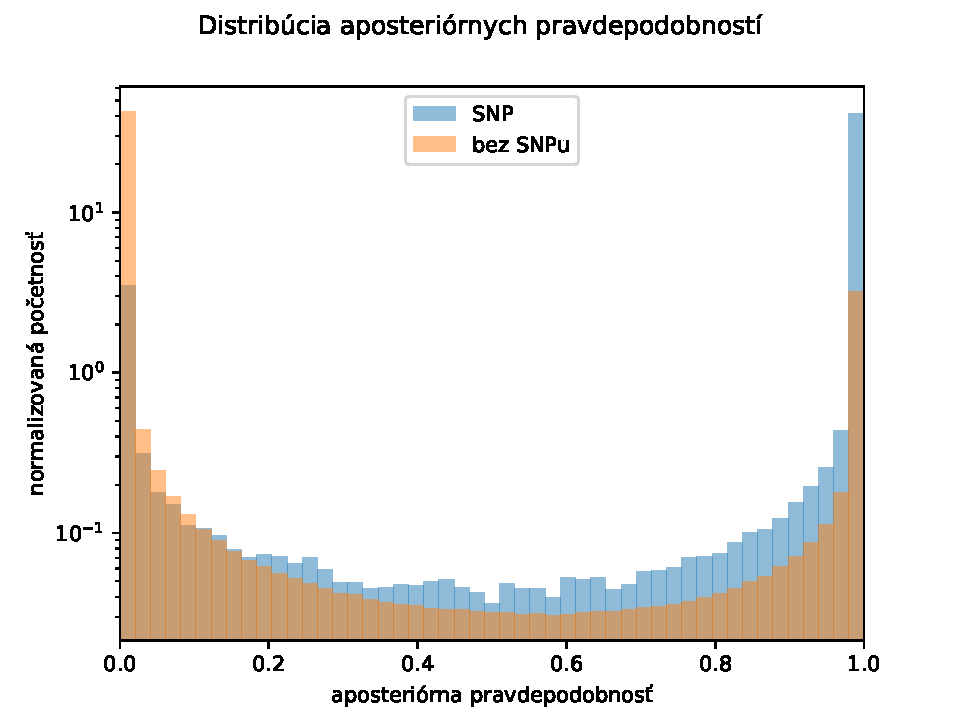
\includegraphics[width=0.7\textwidth]{plots/0_noroot_eqbins}}
\caption[Aposteriórne pravdepodobnosti pre pozície so SNPom a pozície bez SNPu]{Distribúcia aposteriórnych pravdepodobností pre pozície, na ktorých je SNP a pozície, na ktorých nie je SNP. Početnosť
pozícií je normalizovaná a na logaritmickej škále.}
\label{fig:aposteriori_noroot}
\end{figure}


Dá sa teda konštatovať, že náš model si je ,,priveľmi istý'' svojimi predpoveďami. Tento efekt môže
byť spôsobený nerealistickým predpokladom, že jednotlivé merania 
signálu sú nezávislé udalosti. V skutočnosti medzi meraniami pravdepodobne existujú závislosti: keďže
meriame fyzikálnu veličinu v rôznych časoch tesne po sebe, dá sa napríklad očakávať, že v susedných
meraniach väčšinou nameriame podobné hodnoty. Keď teda uvažujeme každé meranie ako samostatnú nezávislú 
udalosť, stáva sa, že podobnú (v podstate tú istú) informáciu model vo svojej predpovedi zohľadní
viackrát.

Viacnásobné zohľadnenie jednej udalosti spôsobuje, že jej prikladá väčšiu výpovednú hodnotu, než táto
udalosť v skutočnosti má. Pri finálnej predpovedi má potom väčšiu istotu, než by mal mať.

Aby sme získali menej extrémne čísla, pred výpočtom aposteriórnych pravdepodobností odmocníme vypočítané 
podmienené pravdepodobnosti desiatou odmocninou. Graf na Obr. \ref{fig:aposteriori_root} ukazuje, ako sa tým
zmení distribúcia aposteriórnych pravdepodobností. Číslo $10$ bolo zvolené na základe predstavy, že
keďže jedna báza je v nanopóre v priemere zhruba počas $10$ meraní, zhruba $10$ po sebe idúcich meraní 
býva podobných a teda jednu udalosť zarátavame v našom modeli zhruba $10$-krát. Tento dôvod je však
čisto intuitívny; aposteriórne pravdepodobnosti, ktoré získame, je preto lepšie chápať iba ako skóre 
určené na porovnávanie dôveryhodnosti hypotéz, nie pravdepodobnosť, s ktorou by sa dali robiť ďalšie 
výpočty. 

\begin{figure}[t]
\centerline{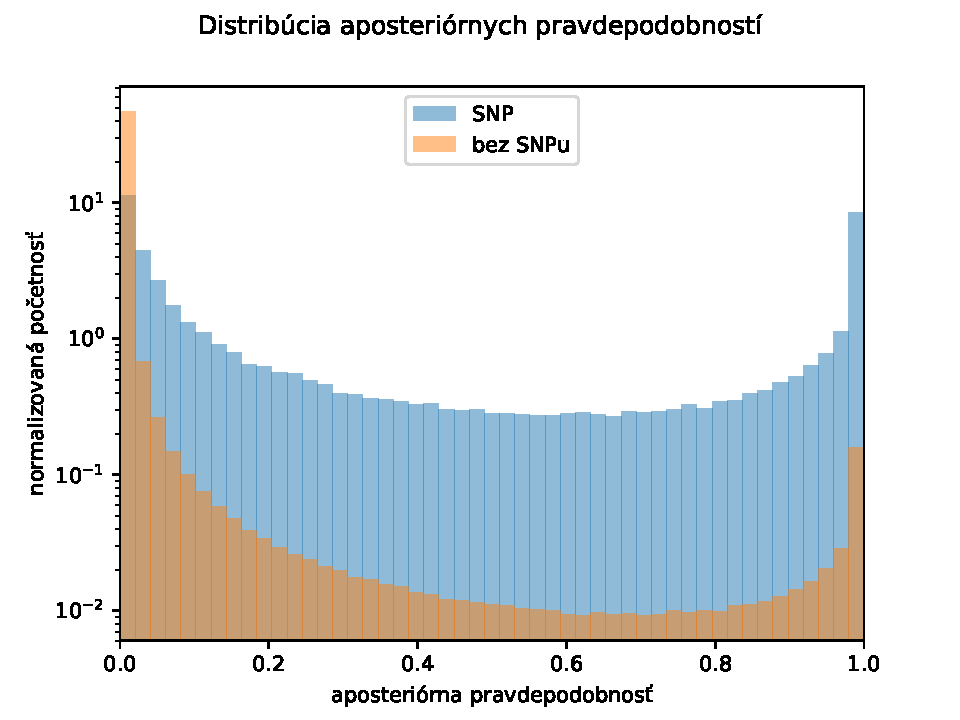
\includegraphics[width=0.7\textwidth]{plots/0_root_eqbins}}
\caption[Aposteriórne pravdepodobnosti pri použití desiatej odmocniny]{Distribúcia aposteriórnych pravdepodobností pri použití desiatej odmocniny.}
\label{fig:aposteriori_root}
\end{figure}

\section{Pozície blízko SNPov}
\label{sec:blizke_pozicie}

Postup, ktorý popisujeme v kapitole \ref{sec:jedna_pozicia} máva často problémy pri pozíciách, na ktorých síce nie je SNP, ale nachádzajú
sa blízko nejakého SNPu. V grafe na Obr. \ref{fig:score_by_SNP_proximity} vidíme, že pozície tesne vedľa SNPov majú vysoké skóre
oveľa častejšie než pozície ďaleko od SNPov, kým pozície ďaleko od SNPov majú oveľa častejšie skóre blízke nule.
Pri týchto pozíciách totiž žiadna zo štyroch uvažovaných hypotéz nezodpovedá realite, nakoľko všetky predpokladajú,
že na pozíciách v okolí skúmanej pozície sa sekvenovaný genóm zhoduje s referenciou.

\todo{obrázok: referencia, reálna sekvencia a 4 hypotézy}

Žiadna z hypotéz potom nedokáže dobre vysvetliť nameraný signál.

\begin{figure}
\centerline{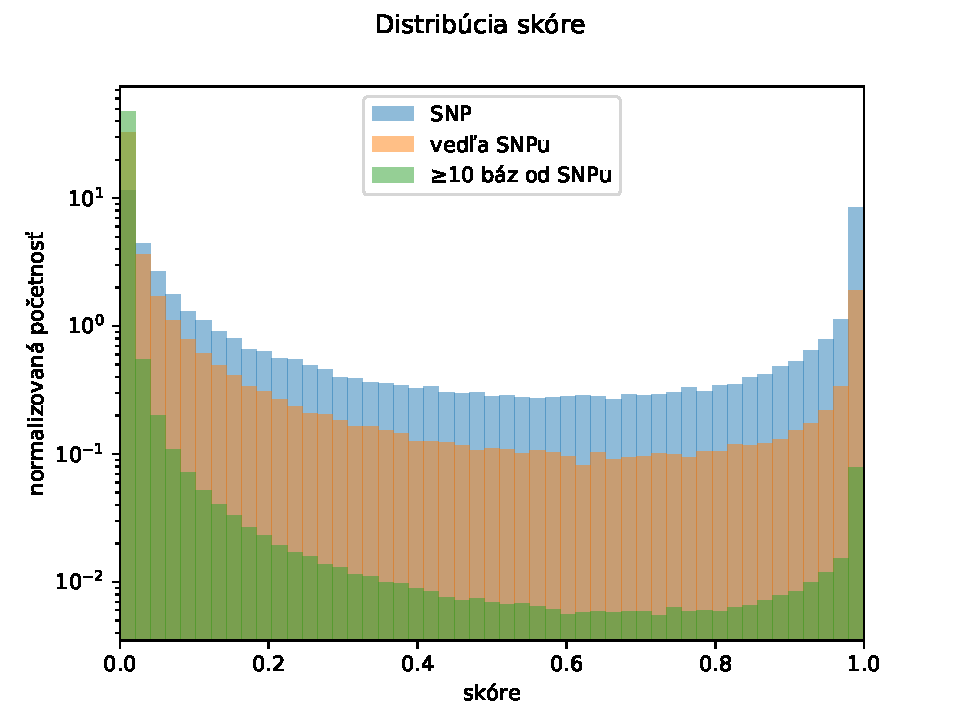
\includegraphics[width=0.7\textwidth]{plots/1_windowed_eqbins}}
\caption[Skóre pozícií so SNPom, vedľa SNPu a ďaleko od SNPu]{Distribúcia skóre pre pozície so SNPom, pozície tesne vedľa SNPu a pozície aspoň desať báz od najbližšieho SNPu.}
\label{fig:score_by_SNP_proximity}
\end{figure}

Tento problém môžeme vyriešiť tak, že pre každú pozíciu berieme do úvahy aj hypotézy, ktoré hovoria, že 
sa SNP nachádza na niektorej z okolitých pozícií. Za okolité pozície pritom považujeme všetky pozície
vzdialené nanajvýš $k-1$ od tej skúmanej, teda všetky pozície, ktoré v našom modeli majú nejaký vplyv
na úsek signálu ovplyvnený skúmanou pozíciou.

\todo{obrázok: sekvencia báz a zarovnaný signál, s vyznačenými časťami signálu ovplyvnenými skúmanou bázou a bázami vzdialenými $k-1$}

Namiesto štyroch hypotéz teda budeme mať $3 \cdot (2k-1) + 1$ hypotéz: jedna hovorí, že v sekvenovanej 
postupnosti nebol v okolí skúmanej pozície žiaden variant, tri hovoria, že na skúmanej pozícii je SNP a
$3 \cdot (2k-2)$ hypotéz hovorí, že na niektorej z okolitých pozícií je SNP.

Pri určovaní apriórnych pravdepodobností hypotéz budeme pracovať s predpokladom, že to, či sa na 
jednotlivých
pozíciách vyskytne SNP, sú nezávislé udalosti.
Ak teda v sekvenovanej postupnosti očakávame podiel SNPov $p$, potom hypotéze, že žiadna z $2k-1$ okolitých 
pozícií neobsahuje variant, priradíme apriórnu pravdepodobnosť $(1-p)^{2k-1}$. Všetkým ostatným 
hypotézam 
priradíme apriórnu pravdepodobnosť $\nicefrac{p}{3} \cdot (1-p)^{2k-2}$, pretože predpokladajú na
práve jednej z $2k-1$ pozícií inú bázu ako referencia. Keďže zanedbávame možnosť, že medzi $2k-1$
bázami by mohol byť viac než jeden SNP, súčet takto vypočítaných apriórnych pravdepodobností pre
naše hypotézy bude menší než $1$. Preto ich nakoniec ešte znormalizujeme: všetky apriórne 
pravdepodobnosti prenásobíme rovnakým číslom tak, aby dávali súčet $1$.


Zvýšením počtu uvažovaných hypotéz sme zvýšili aj čas potrebný na vypočítanie všetkých
podmienených pravdepodobností. Preto navrhneme spôsob, ako náš výpočet zrýchliť.

Časť referencie, ktorá zodpovedá postupnosti sekvenovanej v práve spracovávanom čítaní, označme
$R$. Jej bázy budeme označovať $R_1, R_2, \dots$. Slovom \emph{referencia} budeme v nasledujúcom
texte označovať iba túto relevantnú časť referencie.
Výsek z referencie s ktorým pracujeme, keď odhadujeme, či sa na $i$-tej pozícii v sekvenovanej
DNA nachádza SNP, označme $T^i$. Úsek signálu, ktorý tomuto výseku zodpovedá podľa približného
zarovnania označme $S^i$. Postupnosť, ktorú dostaneme, ak v $T^i$ zmeníme $j$-tu bázu z referencie
na $B$, označme ako $D_{j,B}^i$. Množinu všetkých pozícií, ktoré skúmame, označme $I$ (pôjde o všetky
pozície sekvenovanej postupnosti okrem zopár pozícií blízko začiatku a konca, pre ktoré nemáme
dostatočne dlhý kontext).

V pôvodnom prístupe so štyrmi hypotézami sme pre každé $i \in I, B \in \bazy$ potrebovali vypočítať 
$P(D_{i,B}^i ~|~ S_i)$. V novom prístupe potrebujeme pre každé $i \in I$ vypočítať
$P(T^i ~|~ S_i)$ a pre každé $i \in I; j \in \{i-k+1, \dots, i+k-1\}; B \in \bazy \setminus R_j$ 
potrebujeme vypočítať $P(D_{j, B}^i ~|~ S_i)$. To je $\abs*{I} \cdot (3(2k-1)+1)$ rôznych podmienených
pravdepodobností.

Ak budeme pri každej pozícii ako $T^i$ uvažovať celú referenciu $R$ a ako $S^i$ celý signál (označme
ho $S$), niektoré podmienené pravdepodobnosti sa nám začnú opakovať. Pre každé $i \in I$ bude $P(T^i ~|~ S_i)$
rovné $P(R ~|~ S)$, túto podmienenú pravdepodobnosť nám teda stačí vypočítať len raz. Okrem toho
potrebujeme pre každé $i \in I; j \in \{i-k+1, \dots, i+k-1\}; B \in \bazy \setminus R_j$ vypočítať
$P(D_{j, B}^i ~|~ S_i) = P(R_{j, B} ~|~ S)$, kde $R_{j, B}$ je postupnosť, ktorú dostaneme, ak v
referencii $R$ zmeníme $j$-tu bázu na $B$. Tieto podmienené pravdepodobnosti tiež nie sú všetky rôzne,
stačí nám vlastne vypočítať $P(R_{j, B} ~|~ S)$ pre každé $j \in \{\min(I)-k+1, \dots, \max(I)+k-1\}; B 
\in \bazy \setminus R_j$. Dokopy nám teda stačí vypočítať $3(\abs*{I} + 2k -2) + 1$ rôznych podmienených 
pravdepodobností, čo je zhruba $2k$-krát menej.


Výpočet jednej podmienenej pravdepodobnosti sa nám však výrazne spomalil, keďže sme výšku tabuľky $\mathrm{DP}$, ktorú 
potrebujeme vyplniť, zväčšili na dĺžku celej referencie $R$ a šírku sme zväčšili na dĺžku celého signálu 
$S$. Keďže však pri všetkých podmienených pravdepodobnostiach, ktoré počítame, zarovnávame ten istý
signál k takmer tej istej DNA postupnosti, výpočty si budú veľmi podobné. Tento fakt využijeme nasledujúcim spôsobom.

Dĺžku referencie označme $n$ a dĺžku signálu označme $m$. Postupom z kapitoly \ref{sec:dtw} vypočítame
pre referenciu $R$ a signál $S$
tabuľku $\mathrm{DP}_{R,S}$, ktorej prvok $\mathrm{DP}_{R,S}[y][x]$ je rovný podmienenej pravdepodobnosti,
že by prvých $y$ báz referencie vygenerovalo prvých $x$ hodnôt signálu. Podobnú tabuľku vypočítame aj
odzadu: pre každé $x \in \{0, 1, \dots, m\}, y \in \{0, 1, \dots, n\}$ vypočítame hodnotu $\overline{\mathrm{DP}_{R,S}}[y][x]$,
ktorá bude rovná podmienenej pravdepodobnosti, že by posledných $n-y$ báz referencie vygenerovalo
posledných $m-x$ hodnôt signálu. Pri výpočte $\overline{\mathrm{DP}_{R,S}}$ postupujeme analogicky s 
výpočtom $\mathrm{DP}_{R,S}$, akurát odzadu.

Keď počítame $P(R_{j, B} ~|~ S)$ pre nejaké $j, B$, vypočítame hodnoty $\mathrm{DP}_{R_{j,B},S}[y][x]$ 
iba pre $y \in \{0, 1, \dots, j+c_1+1\}, x \in \{0, 1, \dots, m\}$, teda iba prvých $j+c_1+2$ riadkov 
tabuľky. Okrem toho vypočítame ešte hodnoty $\overline{\mathrm{DP}_{R_{j,B},S}}[y][x]$ pre $y \in \{j
+c_1+1, \dots, n\}, x \in \{0, 1, \dots, m\}$. Podmienenú pravdepodobnosť $P(R_{j, B} ~|~ S)$ potom 
vypočítame ako:

$$P(R_{j,B} ~|~ S) = \sum\limits_{x = 0}^m \mathrm{DP}_{R_{j,B},S}[j+c_1+1][x] \cdot \overline{\mathrm{DP}_{R_{j,B},S}}[j+c_1+1][x]\text{.}$$ 

Pri výpočte $\mathrm{DP}_{R_{j,B},S}$ využijeme, že postupnosť $R_{j,B}$ sa v pozíciách $0$ až $j-1$
zhoduje s referenciou $R$, pre pozície $0$ až $j-c_2-1$ sa teda zhoduje aj \kmer{}, ktorý ovplyvňuje
signál zarovnaný k danej pozícii. To znamená, že tabuľky $\mathrm{DP}_{R,S}$ a 
$\mathrm{DP}_{R_{j,B},S}$ budú mať prvých $j-c_2+1$ riadkov zhodných, teda pre každé $y \in \{0, \dots, j-c_2\}, x \in \{0, \dots, m\}$ bude platiť:

$$\mathrm{DP}_{R_{j,B},S}[y][x] = \mathrm{DP}_{R,S}[y][x]\text{.}$$

Do tabuľky $\mathrm{DP}_{R_{j,B},S}$ nám teda v skutočnosti stačí dopočítať riadky s $y \in \{j-c_2+1, \dots, j+c_1+1\}$, čo je $k$ riadkov.

Pri výpočte $\overline{\mathrm{DP}_{R_{j,B},S}}$ využijeme, že pre všetky pozície od $j+c_1+1$ sa
v $R$ a $R_{j,B}$ zhoduje \kmer{} ovplyvňujúci túto pozíciu, teda tabuľky 
$\overline{\mathrm{DP}_{R, S}}$ a $\overline{\mathrm{DP}_{R_{j,B}, S}}$ sa budú zhodovať v riadkoch s 
$y \in \{j + c_1 + 1, \dots, n\}$. To znamená, že z tabuľky $\overline{\mathrm{DP}_{R_{j,B},S}}$ 
nemusíme počítať nič, všetko už máme vypočítané.

Pri výpočte jednej podmienenej pravdepodobnosti počítame iba $k$ riadkov tabuľky, vyriešili sme
teda spomalenie spôsobené zväčšením počtu riadkov tabuľky. 
Momentálna verzia nášho algoritmu uvažuje všetky možné zarovnania signálu $S$
k sekvenovanej postupnosti. Väčšina zarovnaní je pritom veľmi nerealistických a do výslednej
pravdepodobnosti prispeje len zanedbateľne. Aby sme náš algoritmus urýchlili, obmedzíme sa preto len
na zarovnania blízke približnému zarovnaniu získanému nástrojom \resquiggle{}.

Približné signálové zarovnanie, ktoré sme získali v kapitole \ref{sec:resquiggle} označme $r$. Hodnoty
$\mathrm{DP}[y][x]$ a $\overline{\mathrm{DP}}[y][x]$ budeme počítať iba pre $x, y$, pre ktoré
platí:

$$y \in \{r(x)-5, \dots, r(x)+5\}\text{.}$$

Ostatné hodnoty v tabuľkách budeme považovať za nulové. Tým náš algoritmus obmedzíme na signálové
zarovnania, v ktorých je každá hodnota signálu zarovnaná nanajvýš o $5$ báz inam ako v zarovnaní $r$.
Z každého riadku tabuľky teda budeme počítať iba malú časť, čím vyriešime spomalenie spôsobené
zvýšením počtu stĺpcov tabuľky.

Takéto obmedzovanie počítanej časti tabuľky patrí medzi bežné techniky zrýchľovania
dynamic time warpingu \cite{FastDTW}.

V kapitole \ref{exp:4vsMany} porovnávame tento prístup s pôvodným prístupom popísaným v \ref{sec:jedna_pozicia}.


\section{Vylepšenia zohľadňujúce špecifiká dát}
\label{sec:vylepsenia}
Pri testovaní nášho modelu na reálnych dátach nastávali aj situácie, keď mal problém správne určiť 
prítomnosť SNPu na nejakej pozícii. Skúmaním takýchto situácií sme dospeli k dvom malým vylepšeniam,
ktoré zvýšili presnosť modelu.

\subsection{Doladenie normalizácie}
\label{upg:tweaking}
Jedným z dôvodov, prečo náš model niekedy považoval správnu hypotézu za menej pravdepodobnú než
niektorú z nesprávnych, bol systematický posun skutočného signálu od očakávaného, v rámci celého
čítania. Tento problém sa snažíme riešiť doladením normalizácie signálu.

Na začiatku spracovania každého čítania, po znormalizovaní surového signálu
 tento znormalizovaný signál ešte mierne upravíme.
Pre každú udalosť (úsek signálu) z približného zarovnania vypočítaného nástrojom \resquiggle{} sa
pozrieme na očakávanú priemernú hodnotu signálu v tejto udalosti $e$ a na priemernú hodnotu skutočného
signálu $r$. Dvojice $(r, e)$, pre ktoré je rozdiel $\abs*{r-e}$ väčší ako prah $t=1$ zahodíme.
Ostatné dvojice interpolujeme, snažíme sa teda nájsť takú funkciu $f$, aby pre každú uvažovanú
dvojicu $(r, e)$ platilo $f(r) \approx e$, ale aby funkcia $f$ zároveň bola dostatočne hladká.
Následne každú hodnotu signálu $s$ upravíme na $f(s)$.

\begin{figure}
\centerline{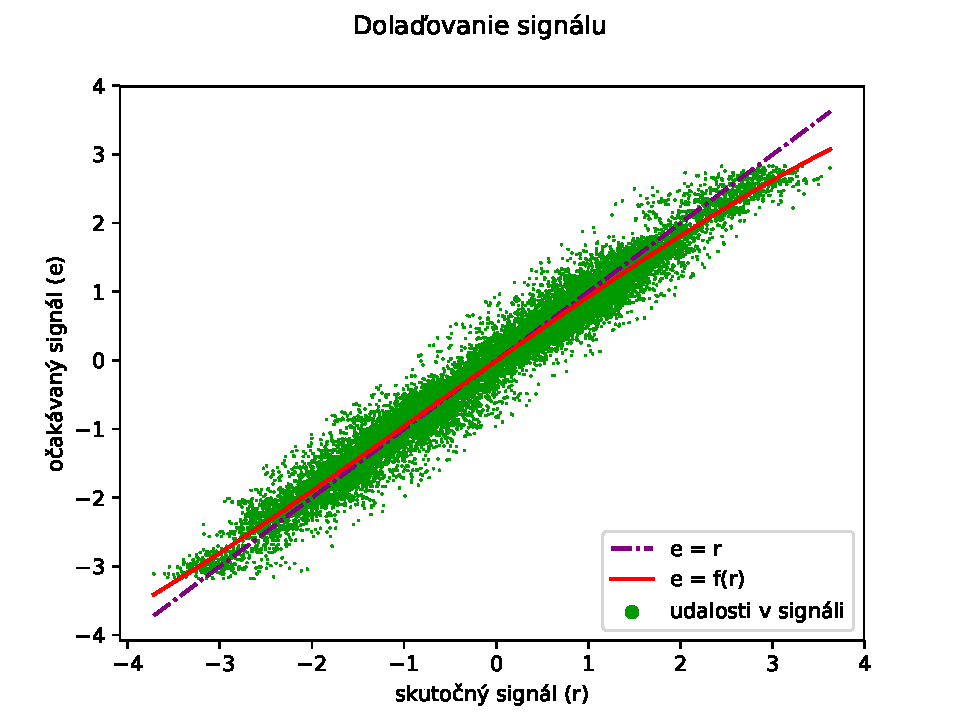
\includegraphics[width=0.7\textwidth]{plots/signal_tweaking}}
\caption{Dvojice $(r, e)$ z jedného čítania, funkcia interpolujúca tieto dvojice a identická funkcia.}
\label{fig:signal_tweaking}
\end{figure}

V praktickej implementácii sme na interpoláciu použili B-spline krivku vypočítanú pythonovskou
funkciou \texttt{scipy.interpolate.splrep}. Graf na Obr. \ref{fig:signal_tweaking} zobrazuje dvojice $(r, e)$
zo signálu jedného čítania, pre ktoré $\abs*{r - e} \leq 1$, funkciu $f$, ktorou sme tieto dvojice interpolovali a identickú funkciu.

Doladenie normalizácie mierne spresnilo náš model, toto spresnenie meriame v kapitole \ref{exp:tweaking}.

\subsection{Modelovanie cúvania}
\label{upg:flashbacks}

V signáli sa občas vyskytuje nasledujúci vzor. Signál sa drží blízko nejakej hladiny $h_1$ a očakávame, 
že po posunutí ďalšej bázy do nanopóru prejde na nejakú inú hladinu $h_2$. Namiesto toho signál 
najprv na krátky čas prejde k hladine $h_2$, potom sa na chvíľu vráti na $h_1$ a až potom naozaj prejde
na hladinu $h_2$, kde už zostane až do ďalšej zmeny spôsobenej posunutím sekvenovaného vlákna v nanopóre.

\todo{Obrázok signálu, pri ktorom pomôže modelovať cúvanie.}

Toto správanie by mohlo byť spôsobené tým, že sekvenované vlákno sa krátku chvíľu hýbe opačným smerom,
pričom sa na chvíľu do nanopóru vráti báza, ktorá z neho práve vyšla. Keďže náš pravdepodobnostný
model s týmto správaním neráta, nevie nájsť dobré signálové zarovnanie ani pre správnu hypotézu.

Preto mierne zmeníme predstavu, ako vlákno prechádza nanopórom. Stále musí platiť, že bázy prechádzajú 
cez
nanopór postupne a každá je tam počas minimálne $M$ po sebe idúcich meraní, medzi každými dvoma
bázami však povolíme ľubovoľne dlhé prechodné obdobie. Od signálu počas prechodného obdobia očakávame, 
že bude v každom momente podobný buď signálu očakávanému tesne pred týmto prechodným obdobím, alebo 
signálu očakávanému tesne po ňom. Rozdelenie pravdepodobnosti pre signál počas prechodného obdobia
definujeme zmiešaním (sčítaním a vydelením dvomi) rozdelenia pravdepodobnosti pre \kmer{}, ktorý bol 
v nanopóre pred týmto prechodným obdobím a rozdelenia pravdepodobnosti pre \kmer{}, ktorý
bude v nanopóre po ňom.

Pozitívny efekt, ktorý mala táto zmena na presnosť nášho modelu meriame v kapitole \ref{exp:flashbacks}.
